\begin{frame}{Comparison Data and Theoritical Calc}
  \begin{tabular}{ccc}
    \begin{minipage}{0.33\hsize}
      \centering
      $\pi^-\Sigma^+$\\
      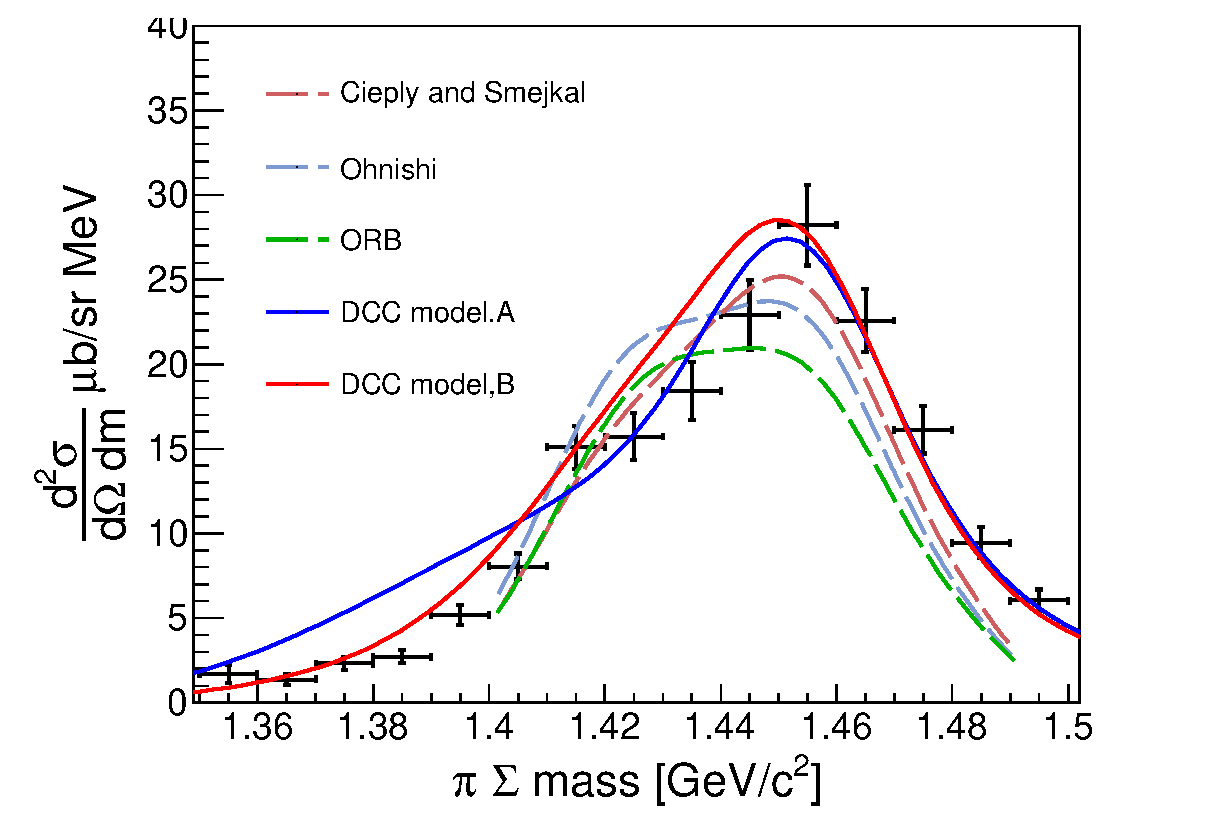
\includegraphics[width=4.3cm]{../pic/Dron/discussion/miyagawa_pimSp.eps}
    \end{minipage}

    \begin{minipage}{0.33\hsize}
      \centering
      $\pi^-\Sigma^+$\\
      \includegraphics[width=4.3cm]{../pic/Dron/discussion/miyagawa_pipSm.eps}
    \end{minipage}
    
    \begin{minipage}{0.33\hsize}
      \centering
      $\pi^-\Sigma^0$\\
      \includegraphics[width=4.3cm]{../pic/Dron/discussion/miyagawa_pimS0.eps}
    \end{minipage}
  \end{tabular}
  \centering
  
  {\footnotesize
    Experimental resolusion is convolved.\\
    Solid and dashed line represent DCC and Miyagawa's calc.
  }
  \vspace{5mm}\\
    
  {
    Absolute value is consistent with data and theoritical calc, \\
    especially DCC.\\
    Model.A can not explained large tail below the threshold.
  } 
\end{frame}
